% =====================================================================
%  G4a - Caliper SATURATION scenario:
%  Request rate progressively increases (200 / 300 / 400 / 500 TPS) across
%  the four round sizes; success rate collapses as the orderer saturates
%  while achieved throughput continues to climb.
%  Source: chapter4.tex Table tab:caliper, saturation columns.
% =====================================================================
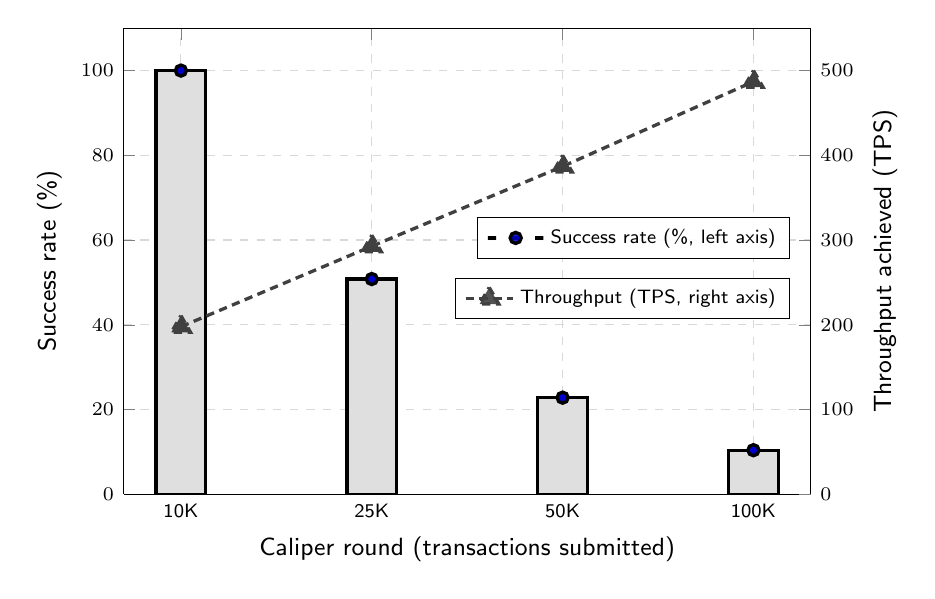
\begin{tikzpicture}
\begin{axis}[
    width=0.85\textwidth,
    height=7.5cm,
    axis y line*=left,
    xlabel={Caliper round (transactions submitted)},
    ylabel={Success rate (\%)},
    ymin=0, ymax=110,
    symbolic x coords={10K, 25K, 50K, 100K},
    xtick=data,
    bar width=18pt,
    grid=major,
    grid style={dashed, gray!30},
    legend style={at={(0.97,0.55)}, anchor=east,
                  font=\sffamily\scriptsize, draw=black,
                  fill=white, fill opacity=0.90, text opacity=1},
    label style={font=\sffamily\small},
    tick label style={font=\sffamily\scriptsize},
]
\addplot+[ybar, fill=gray!25, draw=black, very thick] coordinates {
    (10K,   100.0)
    (25K,    50.8)
    (50K,    22.8)
    (100K,   10.4)
};
\addlegendentry{Success rate (\%, left axis)}
\end{axis}

\begin{axis}[
    width=0.85\textwidth,
    height=7.5cm,
    axis y line*=right,
    axis x line=none,
    ylabel={Throughput achieved (TPS)},
    ymin=0, ymax=550,
    symbolic x coords={10K, 25K, 50K, 100K},
    xtick=data,
    legend style={at={(0.97,0.42)}, anchor=east,
                  font=\sffamily\scriptsize, draw=black,
                  fill=white, fill opacity=0.90, text opacity=1},
    label style={font=\sffamily\small},
    tick label style={font=\sffamily\scriptsize},
    every axis plot/.append style={thick},
]
\addplot+[mark=triangle*, mark size=4pt, color=black!75, mark options={fill=black!75},
          densely dashed, very thick] coordinates {
    (10K,   197.7)
    (25K,   292.7)
    (50K,   386.9)
    (100K,  487.0)
};
\addlegendentry{Throughput (TPS, right axis)}
\end{axis}
\end{tikzpicture}
